\section*{Úvod}
\addcontentsline{toc}{section}{Úvod} 
\indent\indent Cílem mé práce bylo navrhnout a zrealizovat SDR přijímač pro pásmo krátkých vln. Proto bych chtěl v úvodu vysvětlit, copak se za zkratkou SDR skrývá.

Zkratka SDR znamená Software Defined Radio (v překladu Softwarově Definované Rádio). Jedná se o další vývojovou etapu rádiových přijímačů a vysílačů. Analogová rádiová zařízení se postupně vyvíjela od jednoduchých krystalových přijímačů s přímým zesílením, přes přímosměšující tranzistorové přijímače až k velmi složitým přijímačům typu superheterodyn s možnostmi přepínání nejrůznějších demodulací a velkým rozsahem přijímaných pásem. Tyto přijímače ale začínaly být tak složité, že se k napěťovým signálům nesoucím informace mohl v přijímačích přidávat šum. Tento šum zhoršoval  kvalitu přijímaného signálu. SDR je moderní technologie, která se snaží tyto nežádoucí vlivy hardwarových komponentů omezit. Ideální SDR přijímač se skládá jen z antény analogově digitálního převodníku a digitálního obvodu, který signál demoduluje. Díky tomu se k přijímané informaci přidává chyba jen při digitalizaci signálu. Tato technologie tedy posouvá radiová zařízení o světelné roky dál. Jelikož je možné demodulovat v podstatě libovolně modulovaný signál. Přenášet komprimované informace, nebo vytvářet nové digitální modulace. Obrovskou výhodou SDR přijímačů je jejich neustálé vylepšování bez nutnosti jakkoliv měnit hardware přijímače.
\begin{figure}[H]
	\centering
	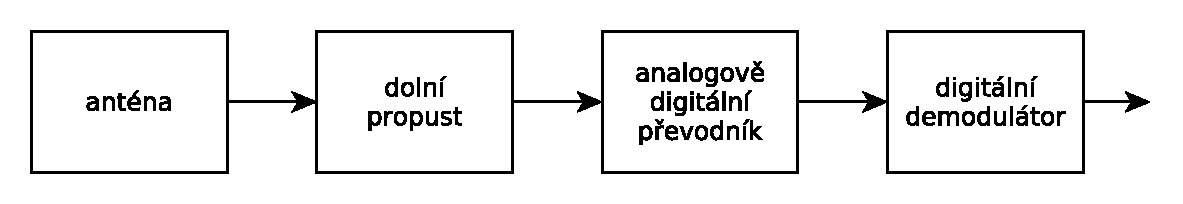
\includegraphics[width=170mm]{img/i_sdr.pdf}
	\caption{blokové schéma ideálního SDR přijímače}    		
\end{figure}

\clearpage
		
	
  		
  		